\section{Validation objective and scope}

This case compares the ELMFIRE reconstruction of the \FireName{} (\FireYear{})
with the GOES-Observed Fire Event Representation (GOFER) arrival-time observation
\cite{liu2024gofer,goferdata}. The event record extends from \EventStart{} to
\EventEnd{}. The simulated quantities are burned extent, fire arrival time,
spread rate and fireline intensity. The comparison evaluates the combined
surface-fire, crown-fire and firebrand-spotting response; it does not isolate
one physical model. Suppression and undocumented interventions are not represented.
No acceptance thresholds were supplied independently of these observations.
An available result is therefore CHARACTERIZED, while missing or unusable results
are NOT EVALUABLE. Prior calibration history is not documented in the supplied
materials; no parameter tuning was performed during preparation of this case.

\section{Reference event, experiment, and observations}

\FireSummary{} The GOFER-derived arrival time is measured in hours since the
GOES ignition hour. Finite cells represent observed burning, and missing cells
represent locations without an observed arrival. This distinction does not
establish that missing cells were unburned at every later time. Satellite
sampling, spatial detection limits and the conversion from hourly perimeters
introduce uncertainty. The exact GOFER version and the complete raster-generation
history are not documented in the available materials.

The observed growth curve below is calculated from the supplied arrival-time
raster. The original hourly vector-area series was not supplied separately for
this case, so the plotted curve must not be interpreted as an independent
second observation. A CAL FIRE Fire and Resource Assessment Program (FRAP)
final perimeter is also supplied as vector geometry and an aligned 30-m burned
mask. The supplied generation source identifies the California Historic Fire
Perimeters release dated 26 May 2026. Its three vector layers retain the
dissolved final perimeter, contributing CAL FIRE records and final GOFER
perimeter. CAL FIRE supplies supporting final-extent information; it does not
supply the hourly arrival times used for the principal numerical comparison.

\begin{figure}[H]
\centering
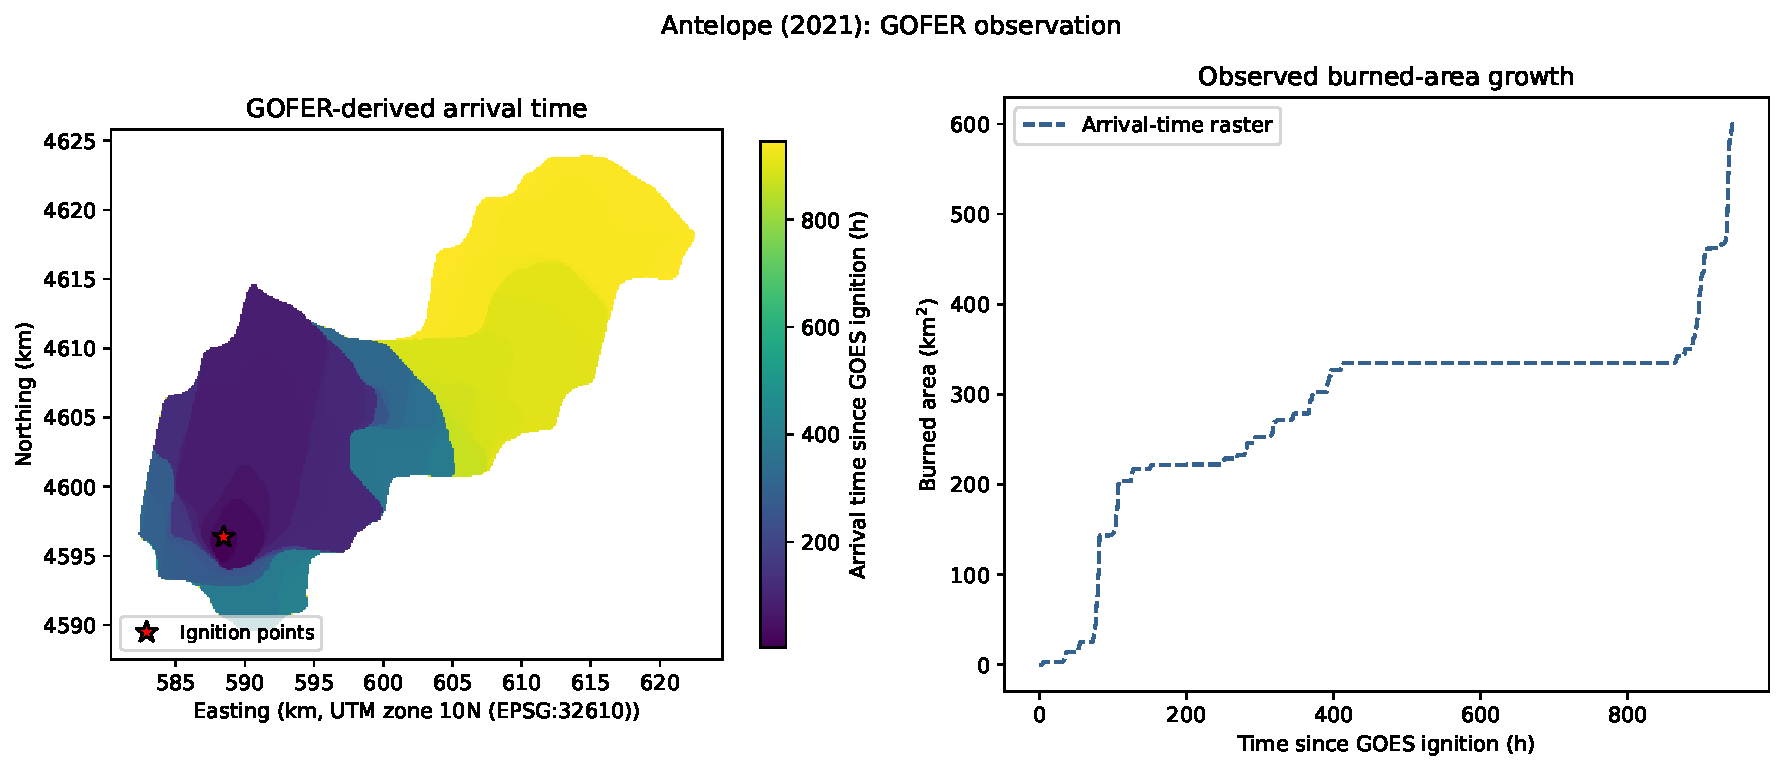
\includegraphics[width=0.98\textwidth,height=0.39\textheight,keepaspectratio]{observation_summary.pdf}
\caption{GOFER observation: spatial arrival time and burned-area growth derived
from the same raster. Times are hours since the GOES ignition hour. Stars mark
used ignition points.}
\end{figure}

\section{Input data provenance and characterization}

\begin{table}[H]
\centering{\small
\begin{tabular}{@{}p{0.22\textwidth}p{0.29\textwidth}p{0.43\textwidth}@{}}
\toprule
Quantity & Source & Interpretation and uncertainty \\
\midrule
Terrain and surface fuels & LANDFIRE, \FuelVersionText{} & 30-m elevation, slope,
aspect and categorical Scott--Burgan fuel model; classification uncertainty is not quantified. \\
Canopy & LANDFIRE, same release & Cover (percent), height and base height (m),
bulk density (kg m$^{-3}$), decoded from scaled integers. \\
Wind and moisture & Historical CloudFire service fields & Hourly wind at 20 ft
(mph and direction from north), dead and live moisture (percent), following
the conventions documented by the supplied preparation source. The underlying
analysis product and moisture derivation are not identified there. \\
Ignition & Supplied GOFER ignition table & Projected positions and elapsed times;
nonburnable-cell adjustments are recorded explicitly. \\
Comparison observations & GOFER and CAL FIRE FRAP & GOFER timed progression;
CAL FIRE supporting final extent. Exact source-version and redistribution gaps
remain recorded. \\
\bottomrule
\end{tabular}}
\caption{Input sources and interpretation. Inputs were supplied on 22 October
2026; this receipt date does not establish their original acquisition dates.}
\end{table}
\ReportBodyText

The domain contains \InputMetric{grid_width} by \InputMetric{grid_height}
cells at \InputMetric{grid_cell_size_m}~m spacing in \CRSName{}, covering
\InputMetric{grid_area_km2}~km$^2$. Elevation ranges from
\InputMetric{dem_minimum} to \InputMetric{dem_maximum}~m; median slope is
\InputMetric{slp_median}$^\circ$. Fuel categories are summarized by area rather
than by numeric averages of model codes. Canopy cover has median
\InputMetric{cc_median}\%, and canopy base height has median
\InputMetric{cbh_median}~m.

\begin{figure}[H]
\centering
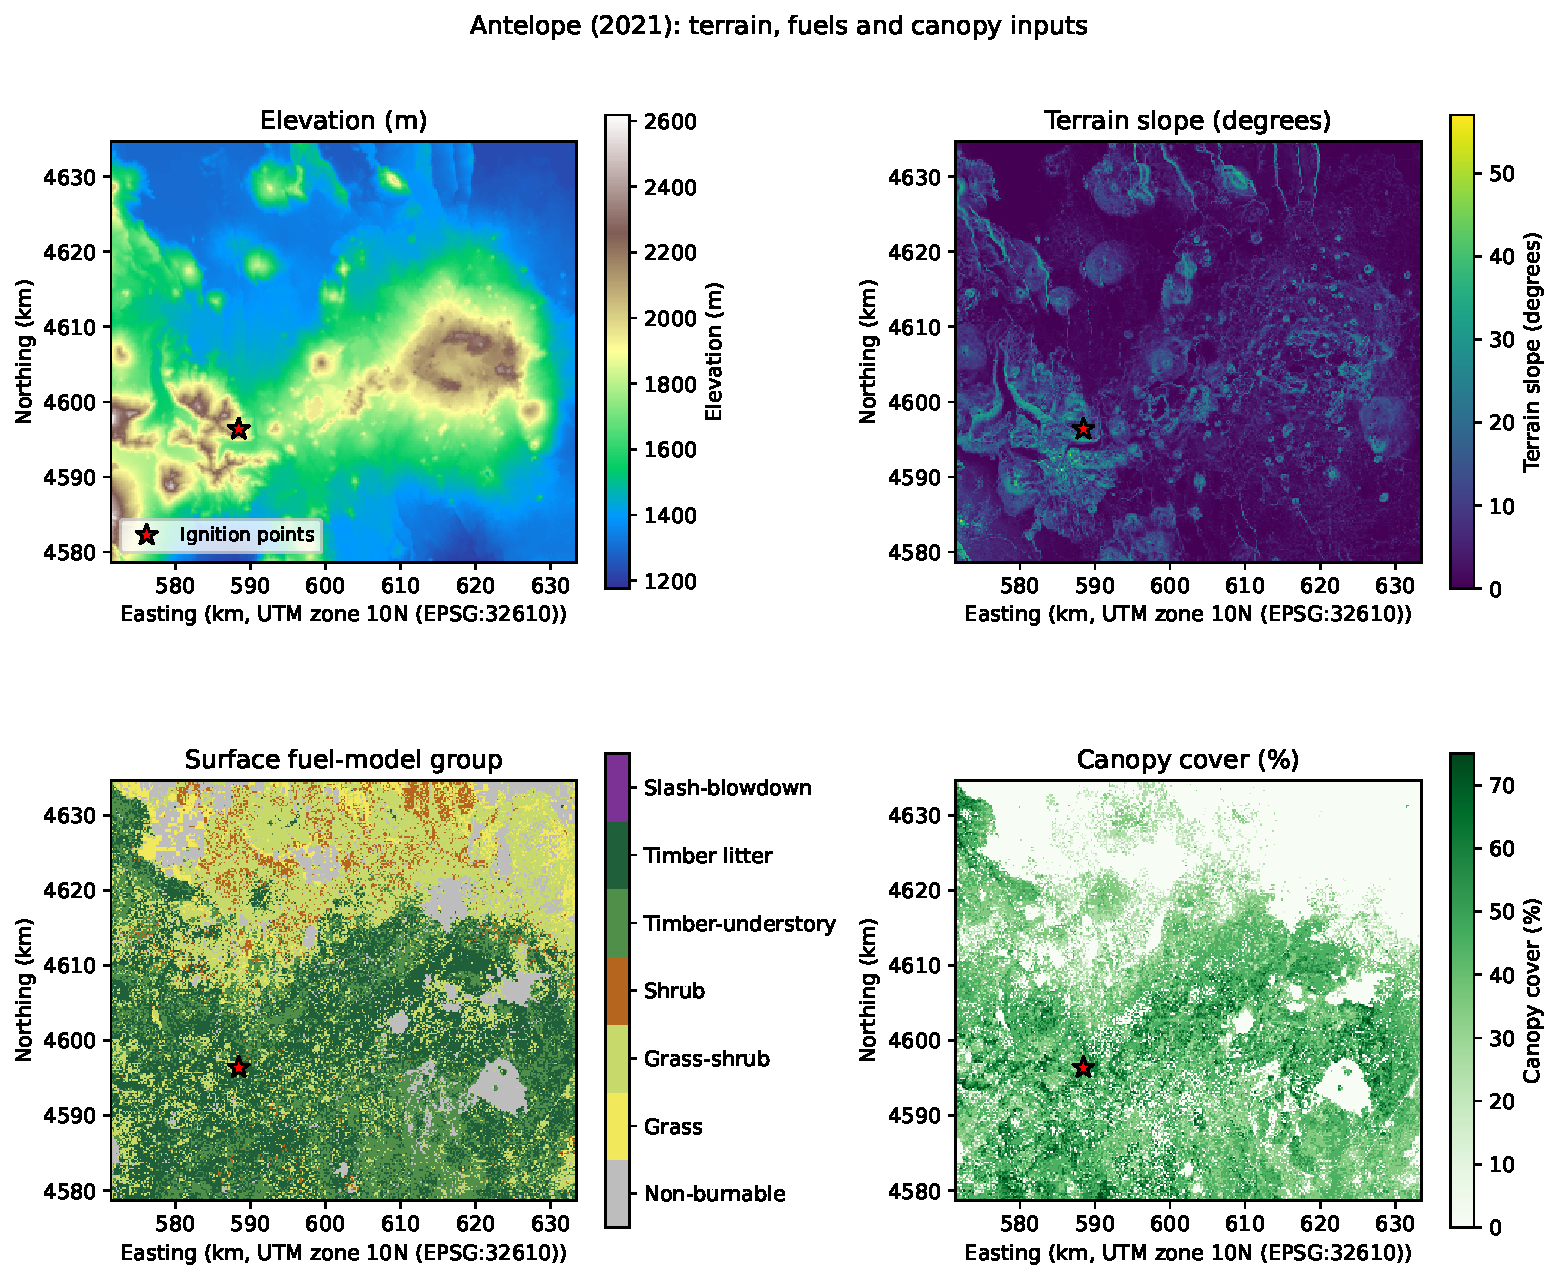
\includegraphics[width=0.92\textwidth,height=0.50\textheight,keepaspectratio]{input_overview.pdf}
\caption{Whole-domain terrain, surface-fuel groups and canopy cover used as model
inputs, with used ignition points. Coordinates are in \CRSName{}.}
\end{figure}
\begin{figure}[H]
\centering
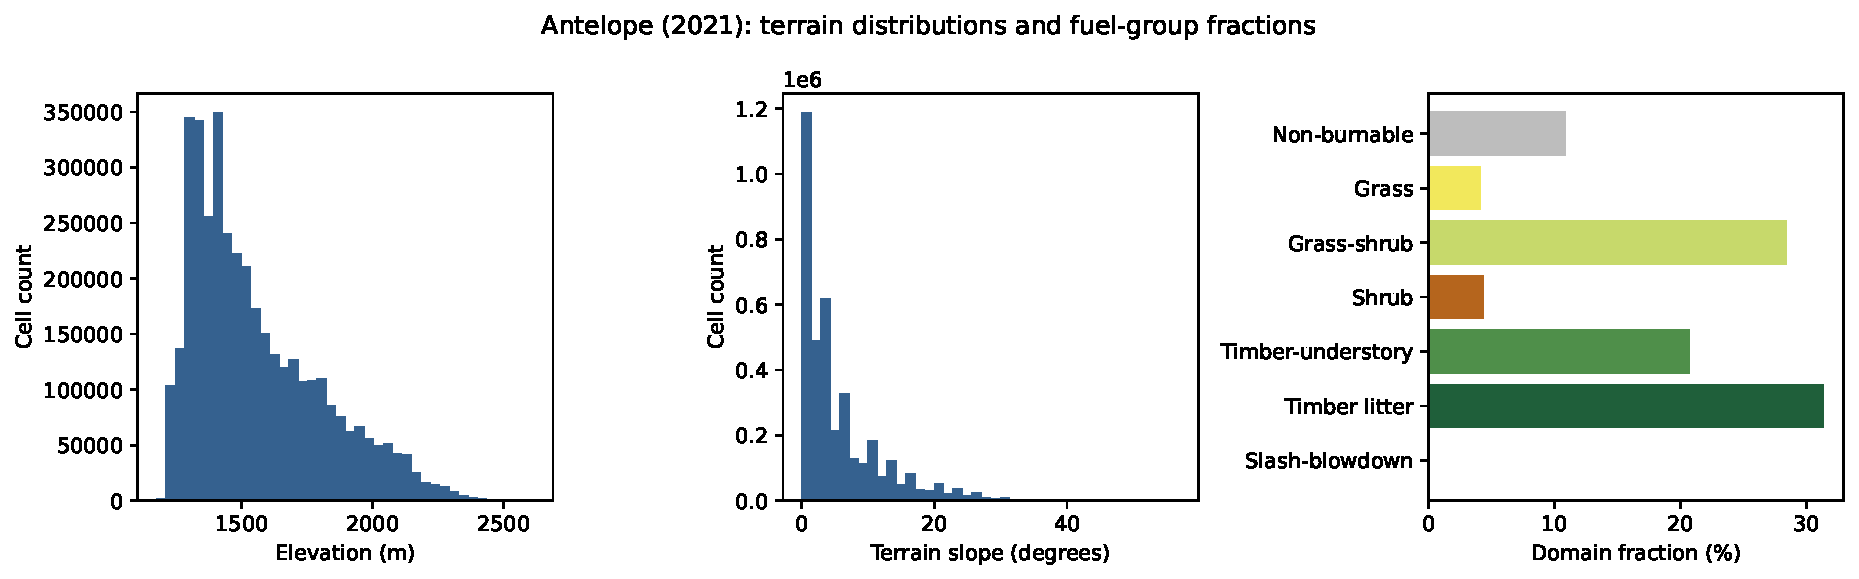
\includegraphics[width=0.98\textwidth,height=0.30\textheight,keepaspectratio]{input_distributions.pdf}
\caption{Input elevation and slope distributions and domain fractions occupied
by surface-fuel groups.}
\end{figure}

The weather contains \InputMetric{weather_bands} hourly fields. Median wind
speed is \InputMetric{ws_median}~mph and its 95th percentile is
\InputMetric{ws_p95}~mph. Direction is summarized circularly: the mean direction
is \InputMetric{wd_circular_mean}$^\circ$ and mean resultant length is
\InputMetric{wd_resultant}. Median 1-h dead-fuel moisture is
\InputMetric{m1_median}\%. Spatial and temporal variability remain important
when these domain summaries are interpreted.

\begin{figure}[H]
\centering
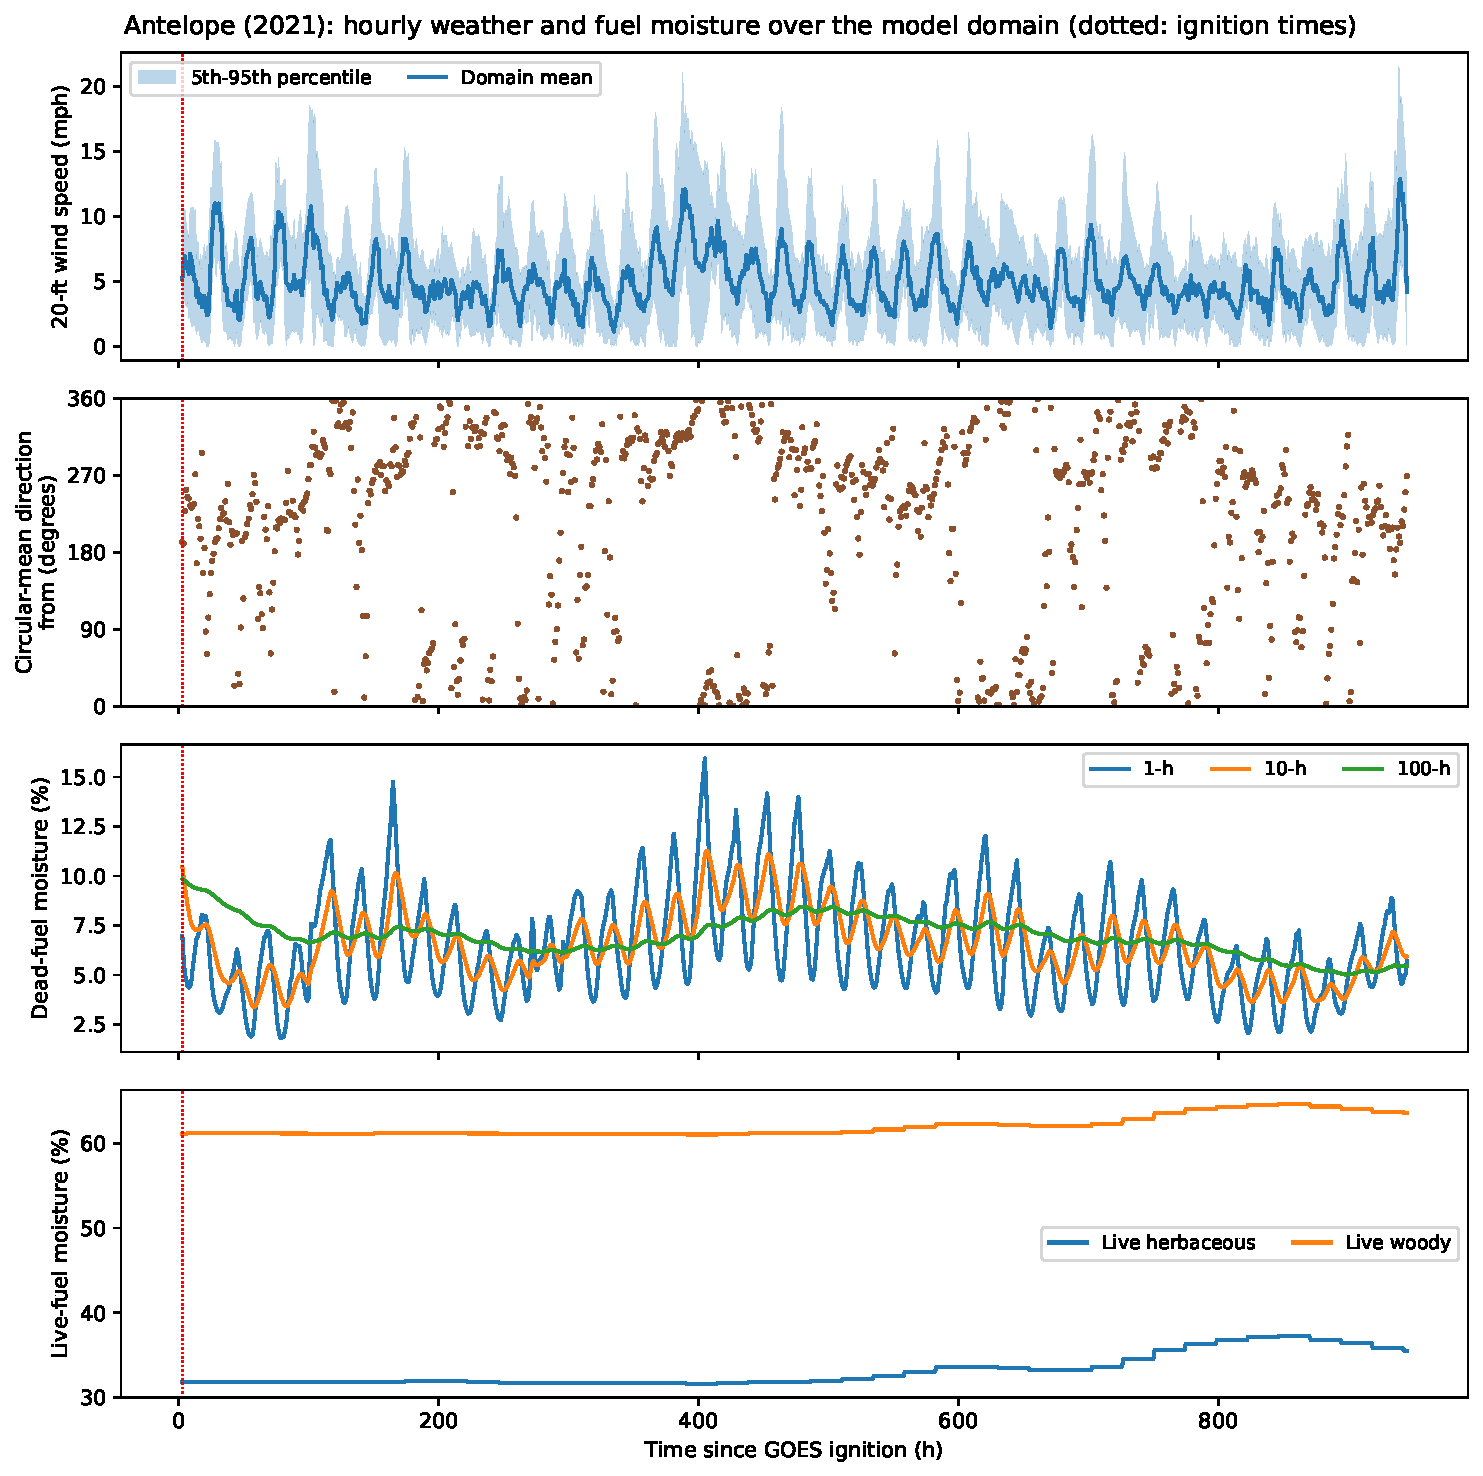
\includegraphics[width=0.96\textwidth,height=0.50\textheight,keepaspectratio]{weather_time_series.pdf}
\caption{Hourly domain summaries of wind and fuel moisture. Wind-speed shading
shows the 5th--95th percentile range; direction uses a circular mean. Dotted
lines mark ignition times.}
\end{figure}
\begin{figure}[H]
\centering
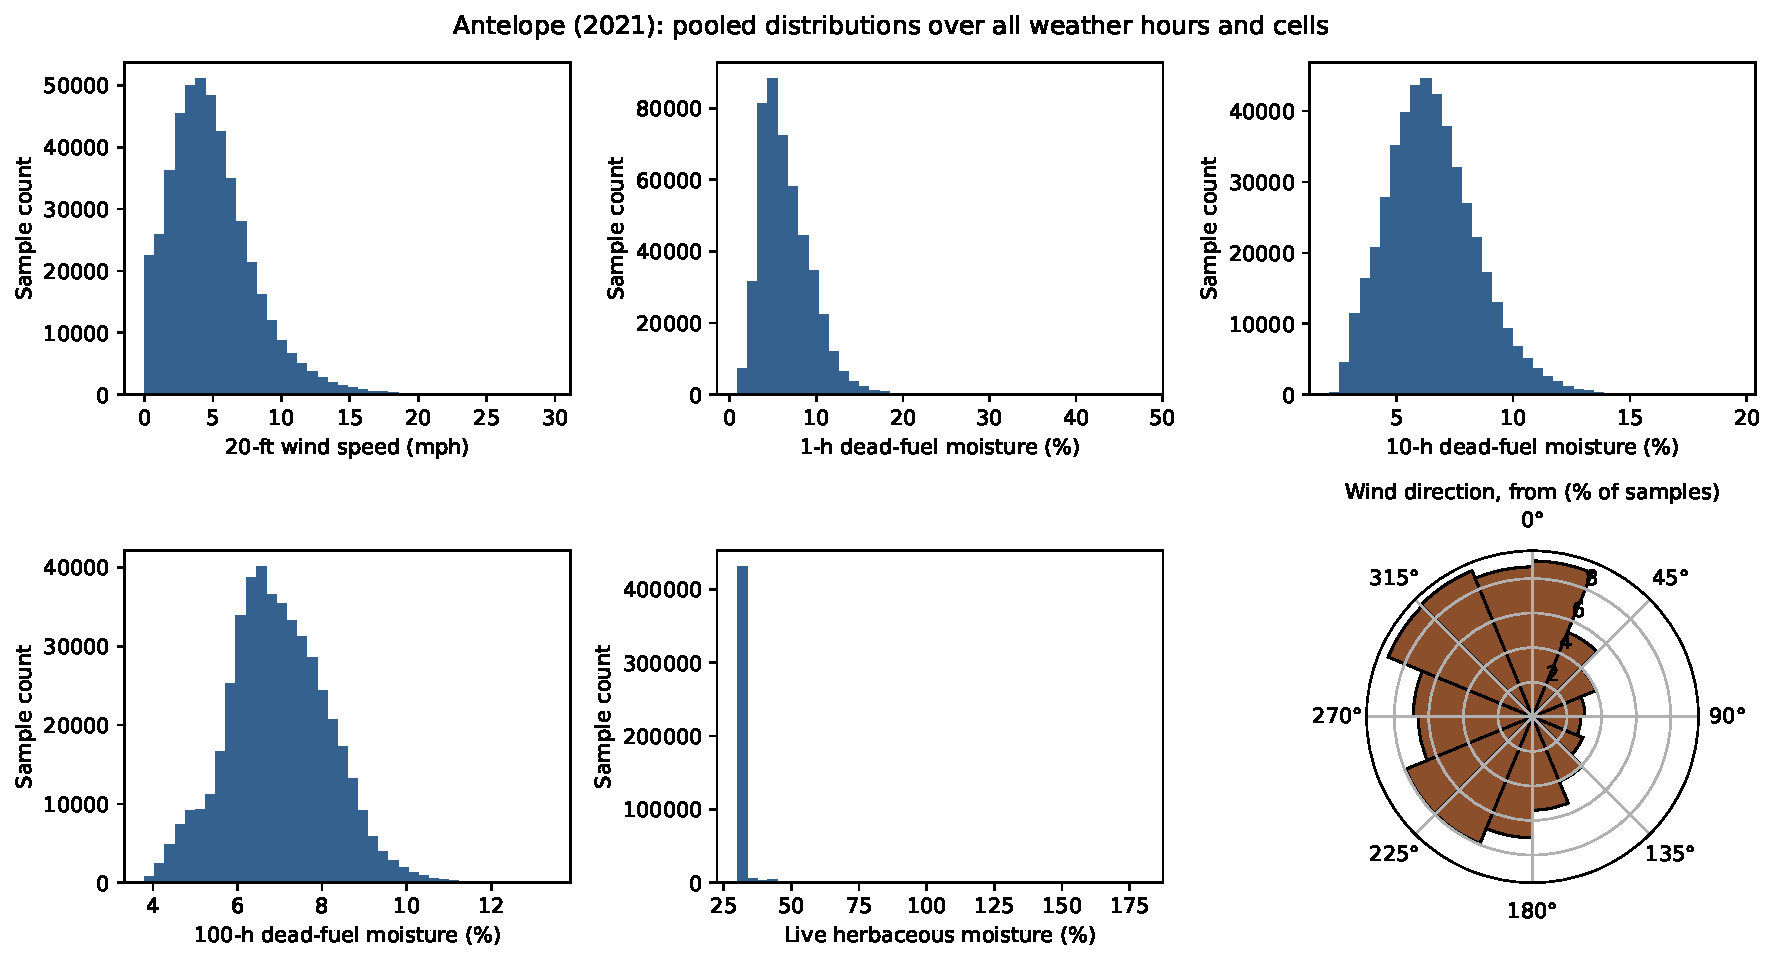
\includegraphics[width=0.97\textwidth,height=0.40\textheight,keepaspectratio]{weather_summary.pdf}
\caption{Weather and moisture distributions from a deterministic spatial sample
at every weather hour, and a wind-direction frequency diagram.}
\end{figure}

\section{Model configuration and rationale}

\ConfigurationText{} The target ELMFIRE source is branch \ElmfireBranch{},
revision \ElmfireRevision{}. The source directory was inspected for accepted
configuration variables, defaults and output conventions. Successful static
checks establish configuration compatibility with that inspected source; they
do not establish executable identity, successful execution or predictive accuracy.

\begin{table}[H]
\centering{\small
\begin{tabular}{@{}p{0.30\textwidth}p{0.18\textwidth}p{0.44\textwidth}@{}}
\toprule
Choice & Basis & Evidence and limitation \\
\midrule
Ignitions and duration & documented & Supplied configuration and ignition table;
all used points and times are retained. \\
Wind and moisture & documented & Supplied hourly rasters and preparation conventions;
underlying analysis and moisture derivation remain incompletely identified. \\
Crown fire and spotting & documented & Supplied configuration retains crown-fire
model 1 and enables spotting; other settings use the inspected source defaults. \\
Timestep and output cadence & documented & Supplied initial timestep, target CFL,
stop time and dump interval are preserved. \\
Acceptance decision & unresolved & No independent numeric thresholds were supplied;
only descriptive characterization is supported. \\
\bottomrule
\end{tabular}}
\caption{Basis of consequential settings and limits on interpretation.}
\end{table}
\ReportBodyText

\section{Preprocessing and reproducibility}

Provided rasters, tables, previews and vector observations are retained unchanged.
Sizes and cryptographic checksums are checked before characterization. The
landscape must contain the eight documented bands. Weather must cover the
landscape, share its coordinate reference system and contain the declared
number of hourly bands. The CAL FIRE burned mask must match the model grid
exactly, contain only burned, unburned or missing-data classes, and agree with
the documented vector-layer coordinate system.

Landscape canopy quantities are decoded using the supplied LANDFIRE scale
conventions. Aspect and wind direction use circular statistics. Observed growth
is the cumulative area of finite arrival-time cells reached by each hour.
\WeatherOffsetText{} A supplied PNG is a preview and is not used as quantitative
evidence. The original data-generation sources are retained, but regeneration
requires external GOFER and CAL FIRE source data and CloudFire access. The
supplied materials do not include the GOFER arrival-time raster generator.

\begin{figure}[H]
\centering
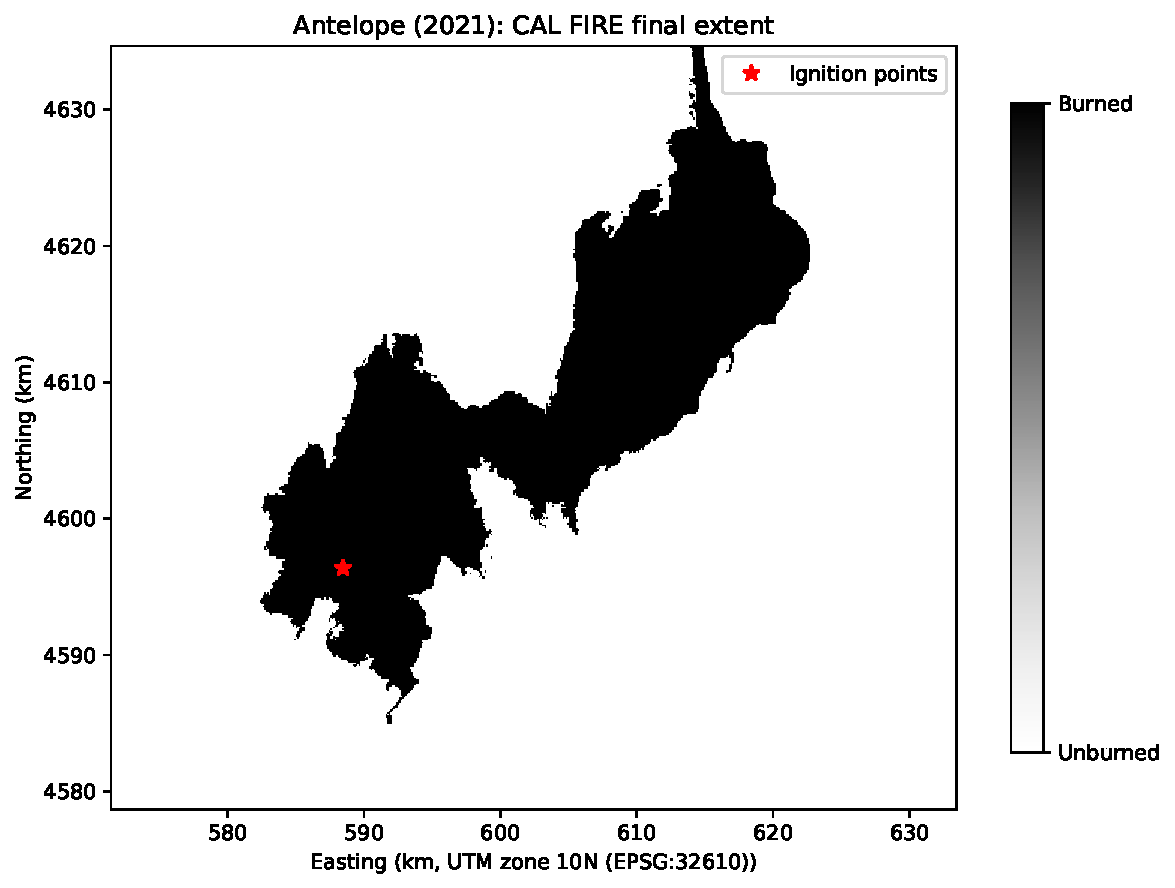
\includegraphics[width=0.86\textwidth,height=0.40\textheight,keepaspectratio]{final_perimeter_summary.pdf}
\caption{Supporting CAL FIRE final extent rasterized at model-cell centres,
with used ignition points. The burned area is
\InputMetric{obs_calfire_burned_area_km2}~km$^2$. This final extent is distinct
from the GOFER timed-progression observation.}
\end{figure}

\section{Validation metrics and comparison method}

The unique latest arrival-time result of simulation member one is selected by
its numeric output time. Negative arrivals are unburned; other values are
converted from seconds since simulation start to hours since the GOES ignition.
The comparison uses every valid landscape cell. Simulated grid coordinates must
match the landscape or the explicitly reproduced single-precision header
rounding of the inspected ELMFIRE source. GOFER times are transferred by nearest
neighbour to these cells; times are not interpolated.

For simulated and observed footprints $S_t$ and $O_t$, let
$I_t=|S_t\cap O_t|$. At 24, 48 and 72~h, when earlier than the last observed
arrival, and at the last observed arrival, report
\begin{align}
J_t&=\frac{I_t}{|S_t\cup O_t|}, &
P_t&=\frac{I_t}{|S_t|}, &
R_t&=\frac{I_t}{|O_t|}, &
F_t&=\frac{2P_tR_t}{P_t+R_t}, &
A_t&=\frac{|S_t|}{|O_t|}.
\end{align}
These are Jaccard overlap, precision, recall, F1 and area ratio. Precision
identifies commission and recall identifies omission; a correct area alone
can hide displacement. Undefined ratios remain unavailable. Within cells burned
in both footprints by the final comparison, report arrival-time bias, mean
absolute error, root mean square error and median error in hours. Growth and
hourly overlap describe the time history. Domain-edge contact and early
termination are reported because they limit the observed simulation history.

The baseline is the supplied GOFER observation, rather than a tuned model run.
Missing or malformed required evidence is NOT EVALUABLE. With valid results,
metrics are CHARACTERIZED because no independent acceptance limits were supplied.
CAL FIRE final extent supplies context and is not substituted for GOFER timing.

\section{Simulation results and field-level comparison}

The current status is \textbf{\Metric{status}}. \Metric{reason}
\SimulationFields{}

\section{Integrated statistics and calculated metrics}

\IntegratedResults{}
\SimulationMetrics{}

\section{Interpretation and uncertainty}

A low overlap with high recall and low precision indicates commission, while
high precision and low recall indicate omission. Neither area agreement nor a
visually similar boundary establishes predictive validity. Satellite sampling,
coarse weather fields, fuel classification, undocumented moisture derivation,
ignition uncertainty, stochastic spotting, omitted suppression and finite domain
extent all affect interpretation. A single realization does not quantify
uncertainty or separate these contributions. The CAL FIRE final perimeter and
GOFER progression can legitimately differ in extent and timing.

\section{Conclusions and limitations}

This case defines a reproducible comparison of the \FireName{} reconstruction
with the supplied GOFER arrival times and characterizes the provided model
inputs and supporting CAL FIRE extent. Its present status is
\textbf{\Metric{status}}, with \Metric{simulations_found} simulation result(s)
evaluated. A defensible acceptance decision requires independently declared
thresholds, documented source and calibration history, and an uncertainty
analysis suitable for the intended application.

\begin{thebibliography}{9}
\bibitem{liu2024gofer} T.~Liu et al., ``Systematically tracking the hourly progression
of large wildfires using GOES satellite observations,'' \emph{Earth System
Science Data}, 16, 1395--1424, 2024,
\href{https://doi.org/10.5194/essd-16-1395-2024}{doi:10.5194/essd-16-1395-2024}.
\bibitem{goferdata} T.~Liu, J.~T. Randerson, Y.~Chen, D.~C. Morton,
E.~B. Wiggins, P.~Smyth, E.~Foufoula-Georgiou, R.~Nadler and O.~Nevo,
GOES-Observed Fire Event Representation product for 28 California wildfires,
Zenodo, \href{https://doi.org/10.5281/zenodo.8327264}{doi:10.5281/zenodo.8327264}.
Exact source version of the supplied arrival times is unverified.
\bibitem{landfire} LANDFIRE, U.S. Department of the Interior, Geological Survey,
and U.S. Department of Agriculture, \href{https://landfire.gov}{landfire.gov}.
\bibitem{calfire} CAL FIRE FRAP, California Historic Fire Perimeters; the supplied
preparation source identifies the release dated 26 May 2026.
\end{thebibliography}
